%!TEX root = ../Studienarbeit.tex

\chapter{Technische Grundlagen}

\section{\acf{HID}}

\subsection{Allgemein}
Das USB Protokoll kann Geräte beim starten beziehungsweie beim einstecken an das System automatisch konfigurieren. Dafür werden Geräte in Klassen eingeteilt. Jede Klasse definiert dabei wie das gewöhnliche Verhalten und die verwendeten Protokolle der Geräte der Klasse sind. Eine dieser Klassen in USB ist die \ac{HID} Klasse. Der primäre Einsatzzweck für Geräte in der \acs{HID} Klasse ist die Bedienung von Computern durch Menschen. Beispiele für solche Geräte sind: Tastaturen, Mäuse, Joysticks, Barcodeleser und auch Simulationsgeräte. \cite[S.~1f.]{usbHIDS}

Informationen eines USB-Geräts für ein Computersystem werden in Segmenten, auch Deskriptoren genannt, des ROMs des jeweiligen USB-Geräts abgespeichert. Ein Gerät, welches sich in der \acs{HID}-Klasse befindet, hat wie in Abbildung \ref{fig:hiddeskriptoren} zu sehen ist drei Deskriptoren. Zunächst einmal den \acs{HID} Deskriptor, welcher alle weiteren benötigte Deskriptoren für USB-\acs{HID}-Geräte auflistet. Der zweite optionale Deskiptor ist der physikalische Deskritpor. Dieser stellt Informationen an das System bereit, wie einzelne Teil des \acs{HID}-Geräts von einen Menschen bedient werden sollen. Dieser wird in dieser Arbeit nicht genauer betrachet. Der letzte Deskriptor ist der Report Deskriptor. Mittels diesem Deskriptor wird die Struktur der übermittelten Daten zwischen dem Rechnersystem und dem \acs{HID}-Gerät beschrieben. \cite[S.~4f.]{usbHIDS}

\begin{figure}[h]
    \centering
    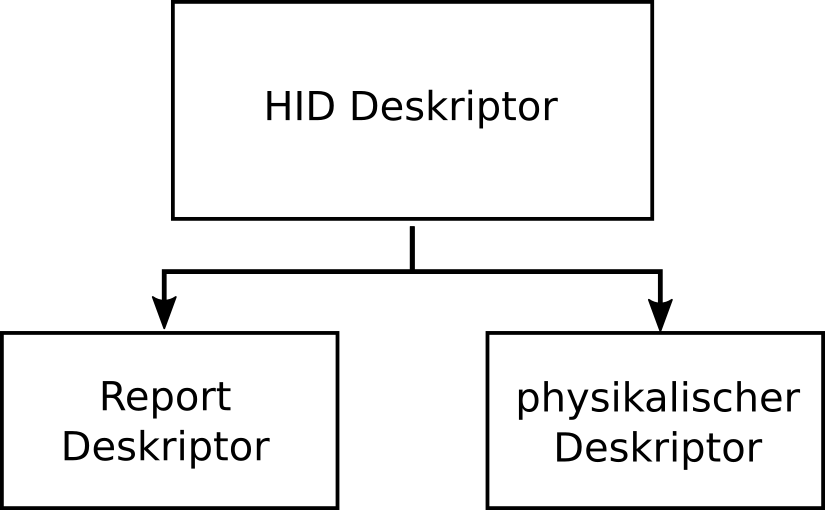
\includegraphics[height=.3\textwidth]{hiddeskriptoren}
    \caption{\acs{HID} Deskriptorenhierarchie; abgewandelt von \cite[S.~4]{usbHIDS}}
    \label{fig:hiddeskriptoren}
\end{figure}

\subsection{Report Deskriptor}

Das USB-Protokoll definiert meist in USB-Geräte-Klassen das zu verwendende Protokoll des Geräts durch Subklassen. Dies ist jedoch in der USB-\acs{HID}-Klasse nicht der Fall. USB-\acs{HID}-Geräte stellen nämlich durch den Report Deskriptor einen anderen System den Aufbau und die Datentypen der übermittelten Datenpakete bereit. \cite[S.~8]{usbHIDS} Durch dieses Verfahren ist es möglich, dass Applikationen durch lesen des Report Deskriptors die modular aufgebauten Daten verarbeiten können \cite[S.~24]{usbHIDS}. Die Länge des Deskriptors ist dabei für jedes Gerät variabel und hängt von der Mänge der übermittelten Daten ab \cite[S.~23]{usbHIDS}.

Ein Report Deskriptor ist dabei aus sogennanten Elementen aufgebaut. Ein Element stellt eine Teilinformation über ein USB-\acs{HID}-Gerät dar. Jedes Element hat zu beginn jeweils ein 1~Byte großes Präfix. In diesem Präfix befinden sich jeweils ein Element-Marker, ein Elementtyp und eine Elementengröße. Darauf folgend können optional Daten angefügt werden. Es kann dabei zwischen langen und kurzen Elementen unterschieden werden, wodurch die Größe zwischen 0 und 258~Byte groß sein kann. \cite[S.~14]{usbHIDS}

Alle benötigten Elemente die in einem Report Deskriptor enthalten sein müssen sind in nachfolgender Aufzählung enthalten: Input (\,Output oder Feature)\,, Usage, Usage\_Page, Logical\_Minimum, Logical\_Maximum, Reprot\_Size und Report Count. \cite[S.~24]{usbHIDS}

Alle Elemente eines Report Deskriptors lassen sich in drei Gruppen einordnen. Zunächst gibt es die Hauptelemente. Diese werden verwendet, um Datenfelder zu definieren oder Datenfelder zu gruppieren. Die zweite Gruppe sind die globalen Elemente. Mit diesen werden die zu übermittelten Datenfelder beschrieben. Die letzte Gruppe umfasst die lokalen Elemente. Diese werden verwendet, um Merkmale eines Datenfelds zu beschreiben. \cite[S.~16, S.~28, S.~35]{usbHIDS}

Die Einsatzzwecke der drei Gruppen stehen folgendermaßen in Beziehung. Mittels eines Hauptelements wird ein Datenfeld definiert. Durch globale und lokale Elemente werden erstellten Datenfeldern Definitionen hinzugefügt. Dabei gelten lokale Elemente nur für das nächst kommende Hauptelement. Globale Elemente gelten im Gegensatz dazu so lange bis das gobale Element durch ein anderes globales Element überschrieben wird. Dadurch ist es möglich Datenstrukturen wie in Abbildung \ref{fig:reportdeskriptorexample} zu erstellen. \cite[S.~24]{usbHIDS}

\begin{figure}[h]
    \centering
    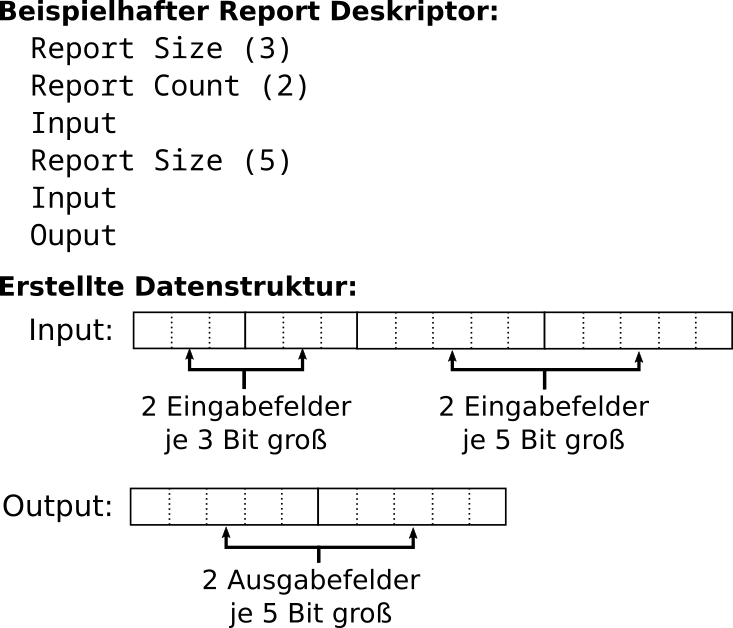
\includegraphics[width=.25\paperheight]{reportdeskriptorexample}
    \caption{Beispielhafte Verwendung von Elementen, um eine Datenstruktur zu definieren; abgewandelt von \cite[S.~24]{usbHIDS}}
    \label{fig:reportdeskriptorexample}
\end{figure}

Unter der Gruppe der Hauptelemete gibt es fünf Element-Marker. Ein häufig verwendeter Marker ist der Input-Marker, mittels diesem können Ausgabedatenfelder definiert werden. Weitere wichtige Element-Marker für Hauptelemente sind Collection und End Collection, womit Datenfelder gruppiert werden können. \cite[S.~23f., S.~30ff.]{usbHIDS}

In der Gruppe der globalen Elemente gibt es 13 Element-Marker. Wichtige Marker hierbei sind: Usage Page, Logical Minimun, Logical Maximum, Report ID, Report Size und Report Count. Mittels dem Marker Report Size wird angegeben wie groß ein Datenfeld in Bits sein soll. Mit dem Marker Report Count wird angegeben wie viele Datenfelder mit den definierten Eigenschaften erstellt werden sollen. Mit dem Marker Report ID ist es möglich mehrere Datenstrukturen innerhalb eines Report Deskriptors zu erstellen und diese eindeutig zu identifizieren \cite[S.~17]{usbHIDS}. \cite[S.~35ff.]{usbHIDS}

Wichtige Element-Marker der Gruppe der lokalen Elemente, welche elf Element-Marker umfasst, sind: Usage, Usage Minimum und Usage Maximum \cite[S.~40]{usbHIDS}. Durch den Element-Marker Usage wird der Einsatzzweck eines Datenfelds definiert. Ebenso können statt einzelnen Datenfeldern auch Kollektionen von Datenfeldern mit Einsatzzwecken markiert werden. Einsatzzwecke sind in Einsatzzweck-Seiten organisiert und werden mit dem Element-Marker Usage Page definiert. Beachtet werden sollte, dass ein Einsatzzweck so spezifisch wie nötig und so allgemein wie möglich gehalten weden sollte, damit das \acs{HID}-Gerät alle gerätespezifischen Eigenschaften bereitstellen kann. \cite[S.~15f.]{usbHIDt}

Schlussendlich können mittels Padding-Bits die enthaltenen Datenfelder byteorientiert ausgerichtet werden. In Tabelle \ref{table:mousedatastructure} ist eine beispielhafte Datenstruktur für eine Maus mit dazugehörigen Report Deskriptor in Quellcode \ref{lst:reportDeskriptor} zu sehen.

\begin{small}
    \begin{longtable}[c]{|p{1.5cm}|p{1.5cm}|p{1.5cm}|p{1.5cm}|p{1.5cm}|p{1.5cm}|p{1cm}|p{1cm}|p{1cm}|}
        \caption{Datenstruktur einer Maus mit drei Knöpfen; abgewandelt von \cite{usbHIDTutorial}}
        \label{table:mousedatastructure}\\
        \hline
        & \textbf{Bit 7} & \textbf{Bit 6} & \textbf{Bit 5} & \textbf{Bit 4} & \textbf{Bit 3} & \textbf{Bit 2} & \textbf{Bit 1} & \textbf{Bit 0} \\
        \hline
        \hline
        \endfirsthead

        \hline
        & \textbf{Bit 7} & \textbf{Bit 6} & \textbf{Bit 5} & \textbf{Bit 4} & \textbf{Bit 3} & \textbf{Bit 2} & \textbf{Bit 1} & \textbf{Bit 0} \\
        \hline
        \hline
        \endhead

        \hline
        \multicolumn{9}{|r|}{Weiter auf der nächsten Seite}\\
        \hline
        \endfoot

        \hline
        \endlastfoot
        
        \textbf{Byte 0} & unbenutzt & unbenutzt & unbenutzt & unbenutzt & unbenutzt & linke Taste & mittlere Taste & rechte Taste \\
        \hline
        \textbf{Byte 1} & \multicolumn{8}{l|}{relative X-Achsen Bewegung als signed Integer} \\
        \hline
        \textbf{Byte 2} & \multicolumn{8}{l|}{relative Y-Achsen Bewegung als signed Integer} \\
    \end{longtable}
\end{small}

\begin{lstlisting}[caption=Report Deskriptor einer Maus mit 3 Knöpfen \cite{usbHIDTutorial}, label={lst:reportDeskriptor}, style=generalStyle]
0x05, 0x01,     //USAGE_PAGE (Generic Desktop)
0x09, 0x02,     //USAGE (Mouse)
0xa1, 0x01,     //COLLECTION (Application)
0x09, 0x01,     //  USAGE (Pointer)
0xa1, 0x00,     //  COLLECTION (Physical)
0x05, 0x09,     //      USAGE_PAGE (Button)
0x19, 0x01,     //      USAGE_MINIMUM (Button 1)
0x29, 0x03,     //      USAGE_MAXIMUM (Button 3)
0x15, 0x00,     //      LOGICAL_MINIMUM (0)
0x25, 0x01,     //      LOGICAL_MAXIMUM (1)
0x95, 0x03,     //      REPORT_COUNT (3)
0x75, 0x01,     //      REPORT_SIZE (1)
0x81, 0x02,     //      INPUT (Data, Var, Abs)
0x95, 0x01,     //      REPORT_COUNT (1)
0x75, 0x05,     //      REPORT_SIZE (5)
0x81, 0x03,     //      INPUT (Cnst, Var, Abs)
0x05, 0x01,     //      USAGE_PAGE (Generic Desktop)
0x09, 0x30,     //      USAGE (X)
0x09, 0x31,     //      USAGE (Y)
0x15, 0x81,     //      LOGICAL_MINIMUM (-127)
0x25, 0x7f,     //      LOGICAL_MAXIMUM (127)
0x75, 0x08,     //      REPORT_SIZE (8)
0x95, 0x02,     //      REPORT_COUNT (2)
0x81, 0x06,     //      INPUT (Data, Var, Rel)
0xc0,           //  END_COLLECTION
0xc0            //END_COLLECTION
\end{lstlisting}

\section{Bluetooth}

\subsection{Allgemein}

Bluetooth ist ein Kurzstreckenkommunikationssystem, bei welchen die Hauptmerkmale auf Robustheit, einen geringen Stromverbrauch und geringe Kosten gelegt wurde. Bluetooth wir in zwei Kategorien aufgeteilt. Die erste Kategorie ist \ac{BBR}. Die zweite Kategorie ist \ac{BLE}. Beide Kategorien beinhalten dabei Mechanismen, um Bluetooth-Geräte zu entdecken, einen Verbindungsaufbau durchzuführen sowie eine Verbindung herzustellen. Das Augenmerk bei \ac{BLE} Produkten liegt dabei auf einen niedrigen Stromverbrauch, was durch eine geringere Datenrate und eine geringere Einschaltdauer während den Datenaustausch als bei \ac{BBR} realisiert wird. Die Übertragungsrate bei \ac{BLE} in der physikalischen Schicht beträgt 2~MB/s. Zu beachten ist, dass ein Bluetooth-Controller entweder \ac{BLE}, \ac{BBR} oder beide Bluetooth-Kategorien unterstützen kann. \cite[S.~187]{bluetoothCore}

Die Übertragungsfrequenz von \ac{BLE} liegt im lizenzfreien 2.4~GHz \acf{ISM}-Band von 2402~MHz bis 2480~MHz \cites[S.~4]{siliconBLE}[S.~190]{bluetoothCore}. Das Frequenzband ist in 40 physikalische Kanäle mit jeweils einer Bandbreite von 2~MHz aufgeteilt, wie in Abbildung \ref{fig:frequenzbandBLE} zu sehen ist \cite[S.~190]{bluetoothCore}. Drei dieser 40 physikalischen Kanäle sind für das sogenannte Advertising vorhanden ()\cite[S.~190]{bluetoothCore}, welches für die Geräteentdeckung, den Verbindungsaufbau und für das Broadcasting von Nachrichten vorhanden ist \cite[S.~4]{siliconBLE}. Die restlichen Kanäle sind für eine allgemeine Datenübertragung vorhanden \cite[S.~190]{bluetoothCore}. Zusätzlich zu der Aufteilung des Frequenzbandes in Kanäle werden Kanäle in Zeiteinheiten aufgeteilt, welche Events genannt werden \cite[S.~190]{bluetoothCore}. Daten werden in Paketen innerhalb eines Events übertragen. Zusätzlich wird bei der Übertragung von Daten Frequenzhopping betrieben, welches zu Beginn jedes Events stattfindet \cite[S.~190f.]{bluetoothCore}. 

\begin{figure}[h]
\centering
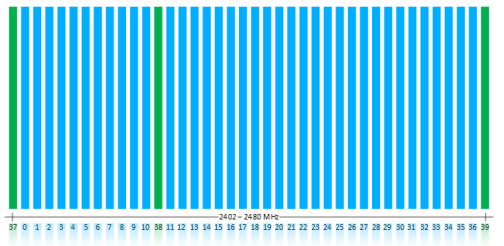
\includegraphics[height=.3\textwidth]{frequenzband}
\caption{Frequenzband mit Kanälen von \ac{BLE}; abgewandelt von \cite[S.~4]{siliconBLE}}
\label{fig:frequenzbandBLE}
\end{figure}

Die Kompatibilität zwischen Bluetooth-Geräten wird durch sogenannte Profile sichergestellt. Profile beschreiben dafür Funktionen und Eigenschaften von jeder Schicht im Bluetoothsystem \cite[S.~277]{bluetoothCore}. Ebenso werden die benötigten Nachrichten und Prozeduren für die verwendeten Profile durch die Bluetooth \ac{SIG} spezifiziert \cite[S.~1241]{bluetoothCore}.

Bluetooth-Geräten werden unterschiedliche Rollen zugewiesen welche entweder Observer, Broadcaster, Central oder Peripheral sein können. Ein Gerät mit der Rolle Broadcaster verschickt Advertising-Pakete und ein Gerät welches nur Advertising-Pakete empfangen kann hat die Observer Rolle. So kann eine einseitige Kommunikation zwischen Geräten mittels Advertising-Paketen erfolgen. Eine andere Art der Kommunikation ist mittels einer Verbindung bei dem das Initiatorgerät eine Verbindungsanfrage eines Broadcastergeräts annimmt. Daraufhin bekommt das Initiatorgerät die Rolle Central und das Gerät welches ursprünglich in der Rolle Broadcaster war, die Rolle Peripherial. Anzumerken ist, dass ein Gerät zu jeder Zeit mehrere Rollen unterstützen kann, welche jedoch alle der Bluetooth-Controller unterstützen muss. \cite[S.~190f., S.~278, S.~1246ff.]{bluetoothCore}

\subsection{Benötigte Komponenten eines \ac{BLE}-Geräts}

Ein \ac{BLE}-Gerät benötigt einen Mindestumfang an Funktionen damit es laut Bluetooth \ac{SIG} \ac{BLE} kompatibel ist. In Abbildung \ref{fig:blestack} sind die benötigten Funktionen und deren Zusammenspiel durch ein Schichtenmodell dargestellt. Die Funktionen können dabei in einen Hostteil und einen Controllerteil aufgeteilt werden. Im Hostteil befinden sich die Funktionen \ac{L2CAP}, \ac{GAP}, \ac{ATT}, \ac{GATT}, \ac{SDP} und \ac{SMP}. Im Controllerteil befinden sich die Funktionen \ac{PHY} und \ac{LL}. Die Kommunikation zwischen den Hostteil und dem Controllerteil finden mittels des \ac{HCI} statt \cite[S.~1735]{bluetoothCore}. \cite[S.~193]{bluetoothCore}

\begin{figure}[h]
    \centering
    \includegraphics[width=.25\paperheight]{blestack}
    \caption{Benötigte Komponenten eines \acs{BLE}-Geräts; abgewandelt von \cite[S.~203, S.~1245]{bluetoothCore}}
    \label{fig:blestack}
\end{figure}

In den nachfolgenden Unterkapiteln werden die wichtigsten Informationen jeder benötigten Funktion von \ac{BLE} beschrieben.

\subsubsection{\acf{PHY}}
Die physikalische Schicht in \ac{BLE} ist zum Verschicken und erhalten von Paketen über eines der physikalischen Funkkanäle verantwortlich. \cite[S.~209]{bluetoothCore}

\subsubsection{\acf{LL}}
Die Verbindungsschicht im \ac{BLE}-System besteht aus mehreren Komponenten. Eine Komponente ist für die Erstellung, Modifizierung und das Freigeben von logischen Verbindungen zuständig. Eine weitere Komponente ist für das Kodieren und Dekodieren von Bluetooth Paketen zuständig. Auch gibt es eine Komponente welche für die Datenflusskontrolle, die Datenbestätigung und für die erneute Übertragen von Paketen zuständig ist. Die letzten Komponenten in der Verbindungsschicht ist für den Zugriff auf das Radiomedium zuständig. Dafür gibt es einen Scheduler, welcher Zeitschlitze des physikalischen Mediums an die höherliegenden Dienste verteilt. \cite[S.~207f.]{bluetoothCore}

\subsubsection{\acf{HCI}}
Das \acl{HCI} stellt die Möglichkeit bereit, dass der Hostteil die Funktionen des Controllerteil erreichen kann. Die Übertragung des \ac{HCI} kann dabei wahlweise mittels USB, UART oder anderen Bussystemen stattfinden. \cite[S.~1735f.]{bluetoothCore}

\subsubsection{\acf{L2CAP}}
Das \acl{L2CAP} ist die Schicht im \ac{BLE}-Stack, welches eine kanalbasierte Abstraktion zu den Applikationen und Diensten der höheren Schichten bereitgestellt. Diese Schicht kümmert sich zusätzlich, um die Segmentierung, den Zusammenbau, das Multi- und Demultiplexing von Daten auf einer beziehungsweise mehreren logischen Verbindungen. \cite[S.~195, S.~1013]{bluetoothCore}

\acl{L2CAP} baut dabei auf dem Konzept von logischen Kanälen auf, wobei jeder Endpunkt eines logischen Kanals einen eindeutigen \ac{CID} hat \cite[S.~1021]{bluetoothCore}. Die logischen Kanäle werden über logische Verbindungen der \ac{LL}-Schicht übertragen \cite[S.~1013]{bluetoothCore}.

\subsubsection{\acf{GAP}}
Das \acl{GAP} beschreibt die Basisfunktionalitäten welche ein \ac{BLE}-Gerät benötigt \cite[S.~207]{bluetoothCore}. Dabei werden alle, in diesem Kapitel vorgestellten Schichten als Mindestanforderung aufgelistet und alle benötigten Fähigkeiten die eine \ac{BLE}-Rolle enthalten muss \cite[S.~277f., S.~1241]{bluetoothCore}. 

Weitere wichtige Eigenschaften die in \ac{GAP} definiert sind, sind zum einen die Bluetooth-Geräteadressen. Die Geräteadresse wird verwendet, um ein Bluetooth-Gerät eindeutig zu identifizieren. Eine weitere Eigenschaft, welche in \ac{GAP} definiert wird, ist der Gerätename. Dieser Name ist eine benutzerfreundliche Zeichenfolge der an entfernten Geräten angezeigt wird. Der Gerätename kann bis zu 248~Byte lang sein und sollte in UTF-8 kodiert sein. Es muss davon ausgegangen werden, dass ein Gerät nur die ersten 40 Zeichen auswerten kann. \cite[S.~1251ff.]{bluetoothCore}

Damit eine Verfolgung von Geräteadressen minimiert werden kann, gibt es in \ac{BLE} zwei Arten von Geräteadressen. Zum einen eine sich verändernde öffentliche Adresse, welche an allen \ac{BLE}-Geräte verschickt wird. Zum anderen gibt es sich nicht verändernde private Adressen, welche von Geräten ausgerechnet werden können, welche schon einmal eine Verbindung mit einen bestimmten Gerät aufgebaut hatten. Damit können Geräte, welche schon einmal mit einem anderen Gerät verbunden waren, überprüfen, ob es sich um ein bereits bekanntes Gerät handelt. \cite[S.~19]{siliconBLE}

Auch wird in \ac{GAP} beschrieben, wie der Bluetooth-Pin für eine Authentifizierung zweier Geräte im Verbindungsmodus aufgebaut sein muss. Die Pin soll sechs Zeichen lang sein und aus Ziffern bestehen. \cite[S.~1253]{bluetoothCore}

Zu guter Letzt, beschreibt \ac{GAP} noch die verschieden Sicherheitsmodi, welche durch die verschiedenen \ac{BLE}-Rollen implementiert sein müssen \cite[S.~1337]{bluetoothCore}.

\subsubsection{\acf{SDP}}
\ac{SDP} stellt die Möglichkeit bereit, die verfügbaren Dienste und die zugehörigen Merkmale eines Bluetooth-Geräts für entfernte Geräte sichtbar zu machen \cite[S.~1173]{bluetoothCore}. Dabei pflegt das Gerät, welches \ac{SDP} bereitstellt, eine Liste aller Dienste und Merkmale des Geräts \cite[S.~1177]{bluetoothCore}.

\subsubsection{\acf{SMP}}
\ac{SMP} definiert Methoden zum Verbindungsaufbau und zum Schlüsselaustausch zwischen Bluetooth-Geräten \cite[S.~1554]{bluetoothCore}. Die gerätespezifischen Schlüssel, werden für die Identifizierung von Geräten und für den verschlüsselten Datenaustausch zwischen Geräten verwendet \cites[S.~1556]{bluetoothCore}[S.~18]{siliconBLE}.

Der Verbindungsaufbau und der dazugehörige Schlüsselaustausch für die Identifizierung der Geräte erfolgt in 3 Phasen. Die erste Phase ist die Anfrage für einen Verbindungsaufbau. Die zweite Phase, welche nach einer erfolgreichen Anfrage erfolgt, ist die Generierung eines Schlüssels mit einer kurzen oder langen Lebenszeit. Die letzte Phase ist die Bereitstellung der generierten Schlüssel an die Gegenstelle. \cite[S.~1556]{bluetoothCore}

Zu beachten ist, dass es verschiedene Möglichkeiten gibt einen Verbindungsaufbau herzustellen, der abhängig von den Sicherheitsansprüchen der Anwendung definiert werden kann \cite[S.~18]{siliconBLE}.

\subsubsection{\acf{ATT}}
\ac{ATT} ist ein Teilnehmer-zu-Teilnehmer Protokoll zwischen zwei Geräten \cite[S.~206]{bluetoothCore}. \ac{ATT} definiert dabei zwei Rollen, den Client und den Server \cite[S.~1410]{bluetoothCore}. \ac{ATT} erlaubt es Geräten -- Clients -- kleine Werte -- sogenannte Attribute \cite[S.~279]{bluetoothCore} -- zu lesen, zu schreiben und zu entdecken, welche sich auf dem Gerät mit der Rolle Server befinden \cite[S.~1409]{bluetoothCore}. Ein Gerät kann simultan in der Rolle Server und Client sein \cite[S.~279]{bluetoothCore}.

Ein Attribut besteht jeweils aus drei Eigenschaften. Die erste Eigenschaft ist der Attribut-Typ, welcher durch eine \acf{UUID} definiert wird und in \ac{SDP} definiert sind. Die zweite Eigenschaft ist der Attribut-Handle. Der Attribut-Handle ist ein einzigartiger Identifikator für ein Attribut auf einem Gerät mit der Rolle Server. Durch das Handle ist ein Attribut eindeutig auf einem Gerät definiert. Die letzte Eigenschaft eines Attributs sind die Berechtigungen, welche durch eine höhere Schicht definiert werden muss. \cite[S.~1410ff.]{bluetoothCore}

Attribut-Handles haben eine Länge von 16~Bit und können durch weitere spezielle Attribute gruppiert werden \cite[S.~1412f.]{bluetoothCore}. Die Entdeckung aller vorhandenen Attribute eines Servers durch einen Client erfolgt durch eine höhere Schicht des \ac{BLE}-Stacks \cite[S.~1410]{bluetoothCore}.

Die hinterlegten Werte eines Attributs bestehen aus einem Oktett-Array mit einer fixen oder variablen Länge \cite[S.~1413]{bluetoothCore}.

\subsubsection{\acf{GATT}}
\ac{GATT} baut auf \ac{ATT} auf und stellt ein Framework für die Daten, welche in \ac{ATT} gespeichert werden, bereit. \ac{GATT} stellt wie \ac{ATT} zwei Rollen -- den Server und den Client -- bereit. Ebenso definiert \ac{GATT} das Format der Daten, welche auf dem \ac{GATT}-Server gespeichert werden dürfen, in sogenannten Profilen. Attribute werden hierfür in Profile, Dienste und Merkmale untergliedert, wie in Abbildung \ref{fig:gattstructure} zu sehen ist. Ein Applikationsprofil besteht aus einen oder mehreren Diensten, um bestimmte definierte Use-Cases abzudecken und definiert darüber hinaus die benötigten Dienste, Merkmale und Attribute \cite[S.~207]{bluetoothCore}. Ein Dienst enthält eine Ansammlung von Merkmalen und kann andere Dienste inkludieren. Ein Merkmal enthält ein Wert, sowie eine Menge von Deskriptoren. Durch diesen Aufbau ist es einen Client möglich die Daten eines bestimmten Profils auszulesen ohne davor den Aufbau der Attribute des Servers kennen zu müssen. \cite[S.~280, S.~1480]{bluetoothCore}

Anzumerken ist, dass jedes Attribut, welches in \ac{ATT} vorhanden ist, entweder in einer Dienstdeklarierung oder in einer Dienstdefinition enthalten sein soll. \cite[S.~1483]{bluetoothCore}

\begin{figure}[h]
    \centering
    \includegraphics[width=.20\paperheight]{gattstructure}
    \caption{\acs{GATT} Hierarchie; abgewandelt von \cite[S.~281]{bluetoothCore}}
    \label{fig:gattstructure}
\end{figure}

Das \ac{GATT}-Profil soll von anderen Profilen als Grundstruktur verwendet werden, damit eine reibungslose Kommunikation zwischen einen Client und Server sichergestellt werden kann, wie in Abbildung \ref{fig:profilhierarchie} zu sehen ist. \cite[S.~1470]{bluetoothCore}

\begin{figure}[h]
    \centering
    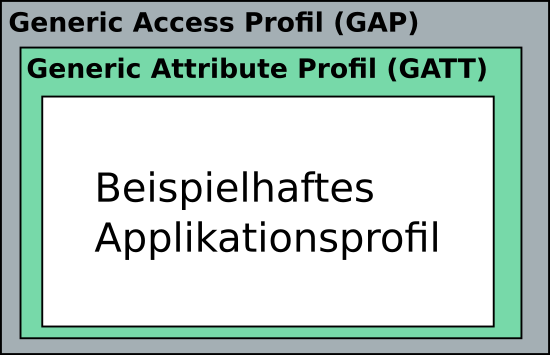
\includegraphics[width=.4\textwidth]{profilhierarchie}
    \caption{Hierarchische Verwendung von Profilen; abgewandelt von \cite[S.~1468]{bluetoothCore}}
    \label{fig:profilhierarchie}
\end{figure}

Ein Dienst stellt unter \ac{GATT} eine Ansammlung von Daten dar, um ein bestimmtes Verhalten durch das vorhandene Gerät darzustellen. Ein Dienst kann zur Vereinfachung der Verhaltensdarstellung weitere Dienste inkludieren. Dienste können in zwei Gruppen eingeteilt werden. Zunächst einmal in die primären Dienste. Primäre Dienste bieten alleinstehende Funktionalitäten an. Im Gegensatz dazu gibt es sekundäre Dienste, welche optionale Funktionalitäten enthalten und von mindestens einen primären Dienst inkludiert werden müssen. \cite[S.~281]{bluetoothCore}

Die Definition eines Dienstes umfasst die inkludierten Dienste sowie die benötigten und optionalen Merkmale \cite[S.~1481]{bluetoothCore}.

Der Start eines Dienstes in der Liste der \ac{ATT}-Attribute wird durch ein spezielles Attribut festgelegt, mit dem Attribut-Typ \textit{primärer Dienst} oder \textit{sekundärer Dienst}. Das Ende eines Dienstes wird durch eine Folgedeklaration eines neuen Dienstes festgelegt. \cite[S.~1483]{bluetoothCore}

Merkmale sind Werte eines Dienstes welche aus mehreren \ac{ATT}-Attributen besteht. Ein Merkmal besteht aus drei Komponenten. Der Deklaration, den Eigenschaften des Merkmals und dem dazugehörigen Wert. Zusätzlich können noch Deskriptoren in einem Merkmal enthalten sein, um die Berechtigungen des Merkmals zu setzen. \cite[S.~281]{bluetoothCore}

Der Start eines Merkmals in der Liste der \ac{ATT}-Attribute wird durch ein spezielles Attribut festgelegt, welche den Attribut-Typ \textit{Merkmal} enthält. Das Ende eines Merkmals stellt eine neue Merkmaldeklaration oder eine neue Dienstdeklaration dar. \cite[S.~1484ff.]{bluetoothCore}

\subsection{Sollanforderungen durch Apple}
Im Apple Ökosystem muss Zubehör welches \ac{MFi} lizenzierte Technologie, zur Verbindung zu Apple Geräte, verwendet -- beispielsweise \ac{MFi} Game Controller -- von Apple geprüft werden. Eine Ausnahme stellen dabei \ac{BLE}-Geräte dar. \cite{appleMfiProgram} Jedoch müssen diese Geräte einige Sollanforderungen in Bezug auf \ac{BLE} erfüllen. Eine Anforderung ist, dass alle drei Advertising-Kanäle bei jeden Advertising-Event verwendet werden sollen \cite[S.~186]{appleDesignGuide}. Dabei muss ein Advertising-Paket mindestens folgende Daten enthalten: TX Power Level, lokaler Name (ohne \textit{:} und \textit{;}), Flags und den Identifikator des primären Dienstes des Geräts \cite[S.~186f.]{appleDesignGuide}. Eine weitere Anforderung ist, dass die Advertising-Intervalle zunächst 20~ms für die ersten 30~Sekunden lang sind und danach auf andere Intervalle umgeschalten werden soll, welche in der Tabelle \cite[S.~187]{appleDesignGuide} stehen. Eine weitere Anforderung ist, dass keine speziellen Berechtigungen benötigt werden, um Dienste und Merkmale eines Gerätes zu entdecken \cite[S.~190]{appleDesignGuide}. Auch soll auf den \ac{BLE}-Geräten der Geräteinformationsdienst implementiert sein, damit der Herstellername, die Modellnummer, die Firmwareversion und die Softwareversion ausgelesen werden kann \cite[S.~191]{appleDesignGuide}. Ebenso sollte Zubehör im \ac{GATT}-Profil das Merkmal mit dem Namen \textit{Gerätename} implementiert haben und durch das Apple-Gerät beschreibbar sein \cite[S.~190]{appleDesignGuide}. Als weitere Anforderung ist zu nennen, dass die Datenpacketlängenerweiterung vorhanden sein sollte, damit der Datenteil eines Pakets statt 27~Byte 251~Byte lang sein kann \cite[S.~189]{appleDesignGuide}. Die letzte Anforderung durch Apple ist, dass \ac{BLE}-Geräte die Fähigkeit besitzen müssen private Geräteadressen auflösen zu können.\cite[S.~189]{appleDesignGuide}.

Auch geben Apple-Geräte nicht alle \ac{BLE}-Dienste an Drittanbieter-Apps weiter, sondern verarbeiten diese intern und geben daraufhin die verarbeiteten Daten an die Drittanbieter-Apps weiter. Die heraus gefilteren Dienste sind: \ac{GAP}, \ac{GATT} sowie \ac{BLE} \ac{HID}. \cite[S.~192]{appleDesignGuide}

\subsection{\acf{HOGP}}
In diesen Abschnitt der Arbeit, wird nur auf die Anforderungen eines \acs{HID}-Geräts -- stellt einen \acs{GATT}-Server bereit \cite[S.~9]{bluetoothHOGP} -- und nicht eines \acs{HID}-Hosts -- stellt einen \acs{GATT}-Client bereit \cite[S.~9]{bluetoothHOGP} -- eingegangen, da eine Implementierung des \acs{HID}-Hosts nicht in diesem Projekt benötigt werden.

Mittels dem \acl{HOGP} werden Prozeduren und Fähigkeiten definiert, welches ein \acs{BLE}-\acs{HID} fähiges Gerät benötigt, um als \acs{HID}-Gerät von \acs{HID}-Host wahrgenommen zu werden. Das Profil baut dabie auf der USB \acs{HID} Spezifikation auf. \cite[S.~9]{bluetoothHOGP}

Das \acf{HOGP} benötigt weitere Profile und Dienste, welche auf einem \acs{HID}-Gerät implementiert sein müssen. Dazu zählen das \acs{GATT}, der Batteriedienst, der Geräteinformationsdienst, das Scan Parameters Profil und der \acs{HID} Dienst. Dabei ist zu beachten, dass auf einem \acs{HID}-Gerät ein oder mehrere Instanzen des \acs{HID}-Dienstes, ein oder mehrere Instanzen des Batteriedienstes, sowie nur eine Instanz des Gerätinformationsdienstes und optional eine Instanz des Scan Parameters Dienstes vorhanden sein darf. \cite[S.~9, S.~11]{bluetoothHOGP} In Abbildung \ref{fig:hidservices} sind alle benötigten und optionalen Dienste grafisch dargestellt. Optionale Dienste werden dabei durch eine gestrichelte Linie angedeutet.

\begin{figure}[h]
    \centering
    \includegraphics[width=.4\textwidth]{hidservices}
    \caption{Benötigte Dienste eines \acs{HID}-Geräts; abgewandelt von \cite[S.~11]{bluetoothHOGP}}
    \label{fig:hidservices}
\end{figure}

Auch werden im \acl{HOGP} für alle benötigten Dienste und Profile zusätzliche Bedingungen festgelegt, welche in den folgenden Unterkapiteln bei dem jeweiligen Dienst beziehungsweise Profil dargelegt sind.

\subsubsection{\ac{HID}-Dienst}

Der \acs{HID}-Dienst ist auf \acs{HID}-Geräten zuständig, um alle benötigten Daten für einen \acs{HID}-Host bereitzustellen. Dabei ist zu beachten, dass alle gespeicherten Merkmale des \acs{GATT}-Servers mit dem niederwertigsten Oktett zuerst übertragen werden müssen. Auch muss der Dienst für den standardkonformen Betrieb mindestens die Merkmale \textit{Report Map}, \textit{HID Information} und \textit{HID Control Point} implementiert haben. \cite[S.~8ff.]{bluetoothHIDS}

\subsubsubsection{Report Merkmal}
Das Merkmal \textit{Report} ist optional. Dieses stellt jedoch ein wichtiges Merkmal dar, da der Datentransfer zwischen \acs{HID}-Gerät und \acs{HID}-Host hauptsächlich über dieses Merkmal stattfindet. Das Merkmal \textit{Report}, kann dabei einen von drei Typen annehmen, nämlich Eingabe, Ausgabe oder Feature. Diese Typen finden sich ebenso in der USB \acs{HID} Spezifikation wieder. \cite[S.~11f.]{bluetoothHIDS}

Da ein \acs{HID}-Gerät mehrere Reports haben kann, muss für jeden Report ein eigenes Merkmal erstellt werden. Zu Unterscheidung der verschiedenen Reports muss jeweils ein Referenz-Merkmalsdeskriptor hinzugefügt werden, welche eine eindeutige Report-ID und den Report-Typen enthält. Als zusätzliche Bedingung müssen in allen Report-Merkmalen vom Typ Eingabe ein Konfigurationsdeskriptor vorhanden sein. Mittels diesen Deskiptor kann konfiguriert werden, ob bei Änderung des Merkmalswerts der \acs{HID}-Host informiert werden soll oder nicht. Der Konfigurationsdeskriptor ist dabei verpflichtend hinzuzufügen. \cite[S.~14.f]{bluetoothHIDS}

\subsubsubsection{Report Map Merkmal}
Im Merkmal \textit{Report Map}, wir der USB Report Deskriptor abgespeichert (wie in der USB \acs{HID} Spezifikation definiert \cite[S.~21]{bluetoothHOGP}), welcher den Aufbau und die Formatierung der einzelnen Report-Merkmale enthält \cite[S.~11]{bluetoothHIDS}. Pro \acs{HID}-Dienst darf jeweils nur eine Instanz dieses Merkmals vorhanden sein und die maximale Größe ist auf 512~Oktette beschränkt \cite[S.~16]{bluetoothHIDS}. Mittels dem zusätzlich benötigten \textit{Report Referenz}-Merkmalsdeskriptors ist es den \acs{HID}-Hosts möglich die Informationen des \textit{Report Map} Merkmals mit den \textit{Report} Merkmalen zu verknüpfen \cite[S.~17]{bluetoothHIDS}.

\subsubsubsection{\ac{HID} Information Merkmal}
Dieses Merkmal enthält eine Ansammlung von Informationen, welche \acs{HID} spezifische Werte sind. Zwei beispielhafte Werte, welche in diesem Merkmal enthalten sind, ist zum einen der Wert \textit{bcdHID}. Dieser wird verwendet, um den \acs{HID}-Host anzuzeigen, welche USB-Spezifikation im \acs{HID}-Gerät implementiert wurde. Zum anderen gibt es den Wert \textit{bCountryCode}. Mit diesem Wert wird angegeben, für welches Land das \acs{HID}-Gerät entwickelt wurde. Da Geräte meist nicht für ein spezielles Land entwickelt werden steht dieser Wert häufig auf 0x00. Das \textit{\acs{HID} Information} Merkmal darf pro \acs{HID} Dienst nur einmal vorkommen und die Daten müssen statisch sein. \cite[S.~20f.]{bluetoothHIDS}

\subsubsubsection{\ac{HID} Control Point Merkmal}
Dieses Merkmal wird von \acs{HID}-Hosts verwendet, um dem \acs{HID}-Gerät anzuzeigen, dass sich der \acs{HID}-Host in den Schlafmodus oder in den normalen Betrieb versetzt. Dieses Merkmal darf nur einmal pro \acs{HID} Dienst vorkommen. \cites[S.~23]{bluetoothHOGP}[S.~21]{bluetoothHIDS}

\subsubsubsection{Zusätzliche Bedingungen durch das \acl{HOGP}}
Alle Merkmale, die in dem \textit{Report Map} Merkmal beschrieben sind und nicht im \acs{HID} Dienst enthalten sind, sollen mittels eines \textit{Includes} in der \acs{HID} Dienst Definition referenziert werden. Zusätzlich müssen alle referenzierten Merkmale den \textit{Report Referenz} Merkmaldeskriptor enthalten. Auch müssen alle \acs{HID}-Dienste als primärer Dienst initialisiert werden und während der Entdeckungsphase für einen Verbindungsaufbau als möglicher Dienst angegeben werden. \cite[S.~13f.]{bluetoothHOGP}

\subsubsection{Batteriedienst}
Mittels diesem Dienst wird dem \acs{GATT}-Host der aktuelle Batteriestatus einer oder mehrerer Batterien des \acs{GATT}-Servers bereitgestellt. Dabei gilt es zu beachten, dass alle bereitgestellten Merkmale des \acs{GATT}-Servers mit dem niederwertigsten Oktett zuerst übertragen werden. \cite[S.~6]{bluetoothBatteryS}

Für diesen Dienst muss ein Merkmal mit den Namen \textit{Battery Level} implementiert werden. Der Batteriestand wird dabei als ein Prozentwert zwischen 0 und 100 angegeben. Wobei 100~\% einer voll aufgeladenen Batterie entspricht. Zusätzlich kann das Merkmal so eingerichtet werden, dass der \acs{GATT}-Server den \acs{GATT}-Client informiert, sobald sich der Wert geändert hat. \cite[S.~8]{bluetoothBatteryS}

\subsubsubsection{Zusätzliche Bedingungen durch das \acl{HOGP}}
Es muss mindestens ein Batteriedienst als primärer Dienst auf dem \acs{HID}-Gerät laufen. Falls ein Batteriestandsmerkmal Bestandteil des \textit{Report Map} Merkmals ist, muss der Dienst mittels eines \textit{Include} in der \acs{HID} Dienst Definition referenziert werden. \cite[S.~14]{bluetoothHOGP}

\subsubsection{Geräteinformationsdienst}
Dieser Dienst stellt einen \acs{GATT}-Client Informationen über den Hersteller und Anbieter des \acs{GATT}-Servers bereit. Dabei darf jedes verfügbare Merkmal nur einmalig pro Dienst vorkommen. Zu beachten ist, dass alle Merkmale optional sind. \cite[S.~6ff.]{bluetoothDeviceI}. In Tabelle \ref{table:deviceinformationlist} sind alle vorhanden Merkmale mit einer kurzen Beschreibung aufgelistet.

\begin{longtable}[c]{|p{4cm}|p{11cm}|}
    \caption{Liste der verfügbaren Geräteinformationsmerkmale}
    \label{table:deviceinformationlist}\\
    \hline
    \textbf{Merkmalname} & \textbf{Kurzbeschreibung}\\
    \hline
    \hline
    \endfirsthead

    \hline
    \textbf{Merkmalname} & \textbf{Kurzbeschreibung}\\
    \hline
    \hline
    \endhead

    \hline
    \multicolumn{2}{|r|}{Weitere Merkmale auf der nächsten Seite}\\
    \hline
    \endfoot

    \hline
    \endlastfoot
    
    Herstellername & Enthält den Namen des Herstellers \cite[S.~8]{bluetoothDeviceI}\\
    \hline
    Modellnummer & Enthält die Modellnummer des Geräteanbieters \cite[S.~8]{bluetoothDeviceI}\\
    \hline
    Seriennummer & Enthält die Seriennummer des Geräts \cite[S.~8]{bluetoothDeviceI}\\
    \hline
    Hardwareversion & Enthält die Hardwareversion \cite[S.~9]{bluetoothDeviceI}\\
    \hline
    Firmwareversion & Enthält die Firmwareversion \cite[S.~9]{bluetoothDeviceI}\\
    \hline
    Softwareversion & Enthält die Softwareversion \cite[S.~9]{bluetoothDeviceI}\\
    \hline
    System-ID & Enthält eine Kombination aus organisatorischer UID und Hersteller definierte ID. Diese ID ist eindeutig für jedes Gerät eines Produkts. \cite[S.~9]{bluetoothDeviceI}\\
    \hline
    IEEE 11073-20601 Regulatory Certification Data Liste & Enthält eine Liste aller Regulations- und Zertifizierungsinfromationen des Produkts \cite[S.~9]{bluetoothDeviceI}\\
    \hline
    PNP-ID & Enthält eine eindeutige Geräte-ID. Diese besteht aus der Anbieter-ID-Quelle (Angabe, ob die Anbieter-ID durch Bluetooth~SIG oder USB Implementer's Forum festgelegt wurde), der Anbieter-ID, der Produkt-ID (von Anbieter festgelegt) und einer Produktversion. Die Produktversion wird als binär-kodierte Dezimalzahl dargestellt. Zum Beispiel Version 2.13 = 0x0213 \cite[S.~10f.]{bluetoothDeviceI}\\
\end{longtable}

\subsubsubsection{Zusätzliche Bedingungen durch das \acl{HOGP}}
Der Dienst muss als primärer Dienst gestartet werden und muss das \textit{PNP-ID} Merkmal enthalten. \cite[S.~14f.]{bluetoothHOGP}

\subsubsection{Scan Parameters Profil}
Mittels diesem optionalen Profil beziehungsweise Dienst, stellt ein \acs{GATT}-Server einen \acs{GATT}-Client Informationen zur Verfügung, die die Geräte unterstützen bei der Verwaltung von Verbindungszeitüberschreitungen und den Advertising Paketen. Durch diese Informationen kann der Stromverbrauch sowie die Wiederverbindungslatenz optimiert werden. \cite[S.~6]{bluetoothScan}

\subsection{Bluetooth-Stacks}

Damit die Verwendung von Bluetooth auf dem verwendeten Mikrocontroller einfacher ist, bietet das \ac{ESP-IDF} zwei Bluetooth-Stacks an. Zum einen den Stack Bluedroid welcher \ac{BBR} und \ac{BLE} unterstützt. Zum anderen wird der Stack NimBLE bereitgestellt welcher nur \ac{BLE} unterstützt. \cite{espidfBluetoothStack}

Bluedroid ist ein von Broadcom Corporation bis 2012 entwickelter Bluetooth-Stack welcher unter der Apache Lizenz steht \cite{bluedroidlizenz}. Dieser Bluetooth-Stack wird von Google seit der Android Version 4.2 als Bluetooth Stack verwendet \cite{lwnBluedroid}. Heutzutage wird dieser Bluetooth-Stack weiterhin unter Android verwendet, aber ist nun unter den Namen Fluoride zu finden \cites{aospFluoride}{anachaoFluoride}.

Apache NimBLE ist ein Open Source \ac{BLE}-Stack, welcher vollständig der Bluetooth~5 Spezifikation konform ist \cite{docnimble} und Bestandteil des Apache Mynewt project ist \cite{gitnimble}.


\section{Übertragungsprotokolle am Fernbedienungsmodulschacht}

Die Multikopter-Fernsteuerungssoftware OpenTX bietet eine Vielzahl von verschiedenen Übertragungsmöglichkeiten zwischen der Fernsteuerung und den Modulen im Modulschacht. Die unterstützten Übertragungsmöglichkeiten sind hierbei: \ac{PPM}, ACCST(D12, D8, LR12)\cite{liangRCProtocols}, DSM, MULTI, ein Protokoll für R9m-Erweiterungsmodule \cite{frskyr9m} und SBUS. \cite{opentxsetup}

Zu beachten bei der Übertragung mittels des PPM-Ausgabepins am Modulschacht ist, dass dieser mittels der Batteriespannung der Fernbedienung betrieben wird, worüber auch das SBUS-Protokoll übertragen wird. Dadurch sollte ein Modul nur betrieben werden, wenn ein Spannungsteiler oder ein Pegelumsetzer vorhanden ist. \cite{opentxFAQ}

Für die vorhandenen Übertragungsprotokolle ACCST, DSM und für das Protokoll der R9m-Erweiterungsmodule konnte keine Dokumentation gefunden werden, weshalb im folgenden Unterabschnitten nur die Übertragungsprotokolle \ac{PPM}, CRSF, SBUS und MULTI betrachtet werden.

\subsection{\acf{PPM}}
\ac{PPM} ist ein Modulationsverfahren, womit Daten -- auch Kanäle genannt -- als Zeitdauer zwischen zwei steigenden Flanken zweier Impulse dargestellt werden, zu sehen in Abbildung \ref{fig:ppmtime}. Ein Paket besteht dabei aus n+1 Impulsen, wobei \textit{n} die Anzahl an Kanälen ist. Nach jedem Paket erfolgt eine Pause von 12~ms, damit eine Synchronisation zwischen Sender und Empfänger gegeben ist. Die Anzahl an Kanälen im Modellbau ist bei \ac{PPM} auf acht Kanäle beschränkt. \cite{hornppm}

Die Gesamtlänge eines Pakets beträgt 22,5~ms mit inkludierter Pause. Die Pulse haben dabei eine Länge zwischen 0,7~ms bis 1,7~ms. \cite{opentxppm}

\begin{figure}[h]
    \centering
    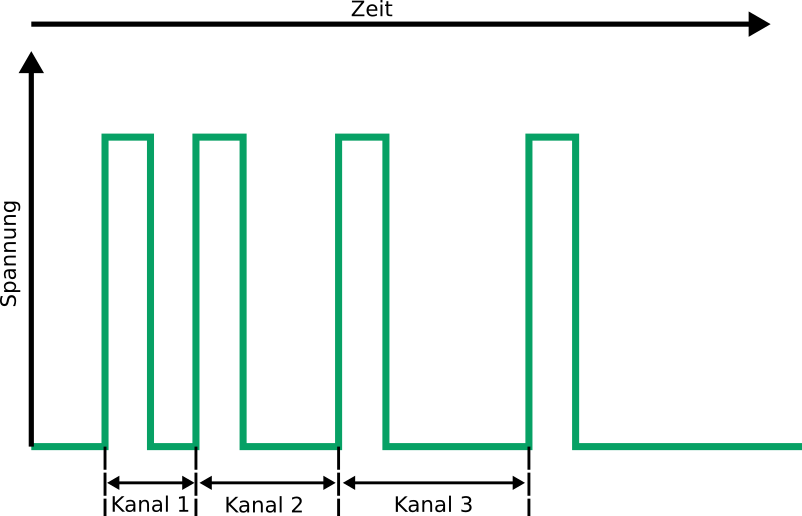
\includegraphics[width=.4\textwidth]{ppm}
    \caption{Darstellung einzelner Kanäle im Zeitverlauf bei \acs{PPM}; abgewandelt von \cite{hornppm}}
    \label{fig:ppmtime}
\end{figure}

\subsection{CRSF}
Das CRSF-Protokoll verwendet eine Eindrahtleitung für eine halbduplex \ac{UART}-Verbindung. Über diese Verbindung sendet der Master alle 6~ms ein Paket. Zwischen den Paketen des Masters kann der Slave den Master optional antworten. Optional zu Beginn eines Pakets gibt es ein Synchronisationsbyte mit den Daten 0xC8. \cites{cleanflightCrsf}{cleanflightCrsfP}

Die Symbolrate beträgt 420000~Baud bei einer 8N1 Übertragung, womit die Übertragungsrate 46~KByte/s entspricht. Bits werden in einer nicht invertierten Weise und Daten werden im Big Endian-Format übertragen. \cite{cleanflightCrsf}

Ein Paket hat eine maximale Größe von 64~Byte und besteht aus fünf Teilen, welche in Tabelle \ref{table:crsfPaket} zu sehen sind. \cite{cleanflightCrsf}

\begin{longtable}[c]{|l|l|l|}
    \caption{Aufbau eines CRSF-Pakets \cite{cleanflightCrsf}}
    \label{table:crsfPaket}\\
    \hline
    \textbf{Feld-Index} & \textbf{Feldtyp} & \textbf{Größe in Byte}\\
    \hline
    \hline
    \endfirsthead

    \hline
    \textbf{Feld-Index} & \textbf{Feldtyp} & \textbf{Größe in Byte}\\
    \hline
    \hline
    \endhead

    \hline
    \multicolumn{3}{|r|}{Weitere Felder auf der nächsten Seite}\\
    \hline
    \endfoot

    \hline
    \endlastfoot
    0 & Geräteadresse & 1\\
    \hline
    1 & Paketlänge & 1\\
    \hline
    2 & Typenfeld & 1\\
    \hline
    3-62 & Daten & maximal 60\\
    \hline
    63 & CRC-Feld & 1\\
\end{longtable}

Die Geräteadressen sind im CRSF-Protokoll vordefiniert. Ein Ausschnitt davon ist in Tabelle \ref{table:crsfAdressen} zu sehen.

\begin{longtable}[c]{|l|l|}
    \caption{Auschnitt aus den vorhandenen CRSF-Geräteadressen \cite{cleanflightCrsfP}}
    \label{table:crsfAdressen}\\
    \hline
    \textbf{Empfängergerät} & \textbf{Adresse}\\
    \hline
    \hline
    \endfirsthead

    \hline
    \textbf{Empfängergerät} & \textbf{Adresse}\\
    \hline
    \hline
    \endhead

    \hline
    \multicolumn{2}{|r|}{Weitere Adressen auf der nächsten Seite}\\
    \hline
    \endfoot

    \hline
    \endlastfoot
    
    CRSF Fernsteuerung & 0xAE \\
    \hline
    CRSF Empfänger & 0xCE \\
    \hline
    CRSF Sender & 0xEE \\
    \hline
    CRSF Multikopterplatine & 0x8C \\
\end{longtable}

Im Paketlängenfeld wird die Größe des Pakets in Byte angegeben, wobei das Typenfeld und das Datenfeld in die Größe des Pakets mit einfließen. \cite{cleanflightCrsf}

Im CRSF-Protokoll werden ebenso wie die Adressen, die Typen fest definiert. Ein Auschnitt möglicher Typen ist in Tabelle \ref{table:crsfTyp} zu finden.

\begin{longtable}[c]{|l|l|}
    \caption{Vordefinierte CRSF Datentypen \cite{cleanflightCrsfP}}
    \label{table:crsfTyp}\\
    \hline
    \textbf{Datentyp} & \textbf{Typenwert}\\
    \hline
    \hline
    \endfirsthead

    \hline
    \textbf{Datentyp} & \textbf{Typenwert}\\
    \hline
    \hline
    \endhead

    \hline
    \multicolumn{2}{|r|}{Weitere Datentypen auf der nächsten Seite}\\
    \hline
    \endfoot

    \hline
    \endlastfoot
    
    Batteriesensor & 0x08 \\
    \hline
    Verbindungsstatistiken & 0x14 \\
    \hline
    Kanaldaten & 0x16 \\
    \hline
    Multikopterflugmodus & 0x21 \\
\end{longtable}

Der Datenteil eines Pakets wird in 16 Kanäle aufgeteilt. Jeder Kanal ist dabei 11~Bit groß. Der Wertebreich pro Kanal liegt zwischen 172 und 1811. \cite{cleanflightCrsf}

Die CRC-Bildung erfolgt über das Typenfeld und das Datenfeld eines Pakets \cite{cleanflightCrsf}. Das Gerneratorpolynom lautet dafür: 0xD5 \cite{cleanflightCRC}

\subsection{SBUS}

Das SBUS-Protokoll ist ein invertiertes (hohes Spannungsniveau = logisch niedrig \cite{sigrokSBus}) serielles Protokoll, über eine Leitung mit einer Symbolrate von 100000~Baud. Die Daten werden dabei im 8E2-Format übertragen. Die Länge eines SBUS-Pakets beträgt 25~Byte mit welchem 18 Kanäle übertragen werden. \cite{BolderFlight}

Das Interval zum versenden von SBUS-Paketen kann in OpenTX zwischen 6~ms und 40~ms frei eingestellt werden. Der Aufbau eines Pakets ist in Tabelle \ref{table:sbusPaket} zu sehen.

\begin{longtable}[c]{|p{3cm}|p{12cm}|}
    \caption{Paketaufbau von SBUS \cite{BolderFlight}}
    \label{table:sbusPaket}\\
    \hline
    \textbf{Byte} & \textbf{Verwendungszweck}\\
    \hline
    \hline
    \endfirsthead

    \hline
    \textbf{Byte} & \textbf{Verwendungszweck}\\
    \hline
    \hline
    \endhead

    \hline
    \multicolumn{2}{|r|}{Weitere Bytefelder auf der nächsten Seite}\\
    \hline
    \endfoot

    \hline
    \endlastfoot
    
    0 & Kopf des Pakets. Immer 0x0F \\
    \hline
    1 - 22 & 16 Kanäle mit jeweils einer Größe von 11~Bit \\
    \hline
    23 Bit 0 & Digitaler ein/aus Kanal 17 \\
    \hline
    23 Bit 1 & Digitaler ein/aus Kanal 18 \\
    \hline
    23 Bit 2 & Paketverlustanzeige. Anzeige, wenn ein Paket zwischen Sender und Empfänger verloren geht. \\
    \hline
    23 Bit 3 & Paketausfallanzeige. Anzeige, wenn mehrere hintereinander verschickte Pakete zwischen Sender und Empfänger verloren gehen. \\
    \hline
    24 & Paketfluss. Immer 0x00 \cite{sigrokSBus} \\
\end{longtable}

Für die Synchronisation zwischen Sender und Empfänger gibt es Lücken innerhalb eines Pakets \cite{sigrokSBus}. Ebenso gibt es eine weitere Version von SBUS, welche den Namen \textit{Fast SBUS} hat und Daten mit einer Symbolrate von 200000~Baud überträgt \cite{BolderFlight}. Der Wertebereich der Kanäle 1 bis 16 liegt zwischen 172 und 1811 und kann auf den Wertebereich von 0 bis 2047 erweitert werden, um die vollen 11 Bit auszunutzen \cite{BolderFlight}. 

\subsection{MULTI}

Das MULTI-Prokoll wird für die Kommunikation zwischen einer Fernsteuerung auf der OpenTX läuft und einem 2,4~GHz Erweiterungsmodul verwendet. Mittels diesem Protokoll wird zum einen das Erweiterungsmodul konfiguriert und zum anderen werden die Daten der 16 zu übertragenden Kanäle an das Erweiterungsmodul geschickt. \cites{langerTransmitter}{langerMultiprotocol}

Die Übertragung findet dabei seriell mittels dem 8E2-Format statt und mit einer Symbolrate von 100000~Baud. In Version~1 ist die Länge eines Pakets 26~Byte. In Version~2 ist die Länge eines Pakets zwischen 27 und 36~Byte groß. \cite{langerMultiprotocol}. In Tabelle \ref{table:mutliPaket} ist der Aufbau eines MULTI-Pakets dargestellt.

\begin{longtable}[c]{|p{2cm}|p{13cm}|}
    \caption{Paketaufbau von MULTI \cite{langerMultiprotocol}}
    \label{table:mutliPaket}\\
    \hline
    \textbf{Byte} & \textbf{Verwendungszweck}\\
    \hline
    \hline
    \endfirsthead

    \hline
    \textbf{Byte} & \textbf{Verwendungszweck}\\
    \hline
    \hline
    \endhead

    \hline
    \multicolumn{2}{|r|}{Weitere Bytefelder auf der nächsten Seite}\\
    \hline
    \endfoot

    \hline
    \endlastfoot
    
    0 & Paketkopf mit der Angabe welche Art von Daten übermittelt werden. \\
    \hline
    1 & Das zu verwendende Protokoll, welches das Erweiterungsmodul zum versenden der Daten verwenden soll. \\
    \hline
    2 & Informationen über den Verbindungszustand zwischen dem Erweiterungsmodul und einem Empfänger sowie das zu verwendende Subprotokoll. \\
    \hline
    3 & Optionale Protokollauswahl, welche nicht verdefiniert ist. \\
    \hline
    4 - 25 & Daten der Kanäle oder die Daten welche bei einen Paketausfall versendet werden. \\
    \hline
    26 & Weitere Protokollinformationen und Telemetriedaten. \\
    \hline
    27 - 35 & Weitere Möglichkeiten zur Protokolldefinition. \\
\end{longtable}

\section{Mikrocontroller ESP}
mehrere Kerne; Pins; Kommunikationsmöglichkeiten; CE z
Zertifizierung (da Antenne schon vorhanden muss nicht erneut zertifiziert werden)

\section{FreeRTOS}
sheduling und Kommunikation zwischen Tasks, interrupts und priorisierung

\section{BITMAP Schriftarten}

\section{libevdev}
